\chapter{Identification and Classification of Uncertainty Regarding Confidentiality}%
\label{ch:classification}%
 

In this chapter, we present the first Contribution \C{1}.
This contribution covers the first two activities shown in \autoref{sec:overview:procedure}, i.e., the identification and classification of uncertainty.
We focus on confidentiality as a central quality property for this thesis.

As introduced in \autoref{ch:introduction}, confidentiality demands that \enquote{information is not made available or disclosed to unauthorized individuals, entities, or processes} \cite{international_organization_for_standardization_isoiec_2018}.
With the growing size and connections of today's software systems, ensuring confidentiality becomes a major challenge. 
We describe in \autoref{ch:overview} that we use design-time confidentiality analysis \cite{seifermann_detecting_2022,tuma_flaws_2019} to identify flaws early and to avoid costly repairs of running systems \cite{boehm_software_2001}.
Here, data flow-oriented analyses became common because \enquote{problems tend to follow the data flow, not the control flow} \cite{shostack_threat_2014}.
However, especially in early development and in complex systems of systems, the software architecture is subject to uncertainty.
This does not only affect decision making---also known as the \emph{cone of uncertainty} \cite{mcconnell_software_1998}---but even blurs which decisions should be prioritized.
When not managed properly, the lack of awareness of uncertainty can void a system's confidentiality.
Also, the \ac{OWASP} Top 10 \cite{OWASPTop10} lists issues like \emph{insecure design} as top security risks.
Thus, we have to actively address the phenomenon of uncertainty and its impact on the confidentiality analysis results.

Managing uncertainty includes activities like the identification and classification \cite{acosta_uncertainty_2022,weyns_introduction_2020,hezavehi_uncertainty_2021}.
Here, multiple taxonomies were defined to better understand the nature of uncertainty \cite{perez-palacin_uncertainties_2014,ramirez_taxonomy_2012,walker_defining_2003}.
However, they mostly originate from the domain of \acfp{SAS} and do not focus on confidentiality.
The consequences are a lack of applicability and an increase in ambiguity.
The relation of software architecture, confidentiality and uncertainty remains unclear \cite{hahner_dealing_2021}.
And while \enquote{there is growing consensus on the importance of uncertainty} \cite{hezavehi_uncertainty_2021}, much is yet unknown regarding the impact of uncertainty on software systems \cite{garlan_software_2010}.
Hezavehi et al. \cite{hezavehi_uncertainty_2021} conducted a survey on uncertainty.
They find a \enquote{lack of systematic approaches for managing uncertainty} \cite{hezavehi_uncertainty_2021} and that uncertainty should already be addressed at design time.
This statement is supported by the work of Troya et al. \cite{troya_uncertainty_2021}.
They conducted a \acf{SLR} and analyzed 123 papers.
They state that \enquote{software models are still falling short of explicitly representing uncertainty} \cite{troya_uncertainty_2021} and that
software engineers require more help \enquote{to identify the types of uncertainty that can affect their application domains} \cite{troya_uncertainty_2021}.

Uncertainty can arise within software systems, e.g., design choices, or reconfiguration at runtime, and their environment, e.g., sensor data, or humans in the loop \cite{acosta_uncertainty_2022,perez-palacin_uncertainties_2014}.
To enhance existing confidentiality analysis approaches, software architects require already known uncertainty sources, which are also called \emph{known unknowns} or first-order uncertainty \cite{perez-palacin_uncertainties_2014}, e.g. known variation of sensors or user behavior.
Second-order uncertainty, also called \emph{unknown unknowns}, cannot be analyzed due to the lack of knowledge about its sources, e.g., due to unforeseen environmental conditions, which limits the development of mitigation strategies \cite{weyns_towards_2023}.
This \acf{UAP} impedes the comprehensive analysis of software systems which poses security threats that could have been resolved at design time.
However, it is a highly subjective phenomenon, as it only depends on the knowledge or awareness of the software architect conducting the analysis. 
Put simply, one cannot analyze what one does not know.

The \ac{UAP} and the related need for collecting uncertainties are supported in the literature.
Recent surveys and research agendas highlight this problem of dealing with unanticipated change \cite{weyns_introduction_2020}, the need to share knowledge of uncertainty \cite{hezavehi_uncertainty_2021}, and the development of \enquote{reusable methods to assess and manage uncertainties} \cite{weyns_towards_2023}.
A class between known and unknown uncertainty was proposed, as not every change is completely unanticipated and can be addressed by flexible designs using intentional over-engineering or meta-adaptation \cite{garlan_unknown_2021}.
To address this, classification approaches alone are not sufficient but require additions like collections and surveys \cite{ramirez_taxonomy_2012,troya_uncertainty_2021}, or expert knowledge \cite{lytra_supporting_2013,esfahani_guidearch_2013}.
Classifications only describe properties of uncertainty which does not resolve the awareness problem, publication-based collections are hard to extend dynamically and are thus prone to become outdated and incomplete, and relying on experts is not expedient.
Developing a joined approach of identification and classification is a step towards end-to-end approaches that promise a higher impact than incrementally enhancing existing analyses \cite{weyns_towards_2023}.

In sum, we aim to address both the identification and classification problem to include uncertainty in confidentiality analysis based on \acfp{DFD}.
This breaks the limitation of previous approaches that were only able to analyze confidentiality with perfect knowledge, i.e., by excluding uncertainty about software systems and their data \cite{seifermann_architectural_2022}.
We summarized this research concern in the first research question:

\RQone

The remainder of this chapter is structured as follows:
First, we summarize the problem statement.
We revisit the relation of uncertainty, confidentiality, and software architecture.
We investigate existing uncertainty classifications and their appropriateness to addressing confidentiality.
Then, we define a new classification of uncertainty regarding confidentiality and discuss, based on this classification, how to represent uncertainty in data flow diagrams.
Afterward, we build on the classification to present an uncertainty catalog approach that helps in the identification of uncertainty and addresses the \ac{UAP}.
We close the chapter with known assumptions and limitations, and also a summary and an outlook.

\ownpublications{
\fancycite{hahner_dealing_2021},
\fancycite{hahner_architectural_2021},
\fancycite{acosta_uncertainty_2022},
\fancycite{hahner_classification_2023},
\fancycite{hahner_arcn_2024}
}





\section{Problem Statement}%
\label{sec:classification:problem}

We summarize the problems \textbf{P1} -- \textbf{P5} addressed by Contribution \C{1}.
Finding solutions to these problems helps to provide a comprehensive answer to \RQ{1}.

\paragraph{P1: Knowledge about the relation of uncertainty and confidentiality}\label{p:1:1}
We need to better understand the role of uncertainty and its relation to confidentiality in software architecture.
This includes considering uncertainty at design time and runtime and also relating uncertainty to \acfp{ADD}, which is related to architectural decision-making under uncertainty \cite{lytra_supporting_2013}.
We see this as a precondition to defining precise classifications of uncertainty regarding confidentiality \cite{hahner_dealing_2021}.
The solution to this problem is considered to be non-trivial due to the variety of uncertainty.

\paragraph{P2: Classification of uncertainty tailored to confidentiality}\label{p:1:2}
We require classifications tailored to confidentiality and software architecture.
There exist classifications from other domains \cite{perez-palacin_uncertainties_2014,ramirez_taxonomy_2012,walker_defining_2003}, but they fall short in representing the impact of uncertainty on confidentiality.
Additionally, they do not relate the classified uncertainty to software architecture and \acp{ADD}.
Here, a classification scheme to aid software architects in understanding the impact of uncertainty on confidentiality. 
This shall raise awareness of properties of uncertainty and their relevance for choosing appropriate \acp{ADD} and mitigation strategies. 
We intentionally speak of a classification rather than a taxonomy because we focus on a subset of uncertainty, i.e., known uncertainty on architectural abstraction.

\paragraph{P3: Representation of uncertainty as first-class concern in \acp{DFD}}\label{p:1:3}
\textcite{garlan_software_2010} raised the need to represent uncertainty as a first-class concern in the design of software systems.
This applies to \acp{ADL} as well as to \acp{DFD}.
Whether in tool-supported analysis or in discussions between software architects, uncertainty must be represented appropriately to be taken into account.
This includes defining a notation for uncertainty impact in \acp{DFD} that works for all uncertainty types of the classification.
Only limited work towards considering uncertainty in \acp{DFD} exists \cite{durugbo_data_2010}, which only considers selected uncertainty types.

\paragraph{P4: Expert knowledge required to understand uncertainty sources}\label{p:1:4}
Due to space limitations in publications, previous approaches only explain classifications briefly without comprehensive data sets \cite{ramirez_taxonomy_2012}.
We stress the importance of explainability \cite{bersani_conceptual_2023}, e.g., using examples, interactive visualizations, and context information from the underlying classification.
Additionally, classifications provide dimensions or categories to describe uncertainties but often fall short in relating multiple uncertainty types which impairs usability \cite{hahner_classification_2023}.
It should be possible to filter, search, and navigate between uncertainties, which requires defined relations between them.
This is especially relevant as uncertainty sources are rarely independent and interactions can occur \cite{camara_uncertainty_2024}.
We do not require an \emph{uncertainty expert} role in our procedure, see \autoref{sec:overview:procedure}.
Therefore, our contributions to the identification and classification must be understandable without extensive training.

\paragraph{P5: Extensible uncertainty source catalogs to support the identification}\label{p:1:5}
The \acf{UAP} states that we need awareness of uncertainty sources to consider them in the uncertainty mitigation process.
One approach to this problem is a collection of uncertainty sources, building on the solutions to the aforementioned problems.
However, publication-based collections are hard to reuse and extend \cite{ramirez_taxonomy_2012} and thus prone to become outdated and incomplete.
Knowledge can be scattered between researchers or organizations which complicates collaboration \cite{sterz_intelligente_2022}.
Additionally, research artifacts often are unavailable \cite{konersmann_evaluation_2022} or partially broken \cite{gerdes_decision_2015,colesky_system_2018}.
To address this, an open-source and publicly available catalog is required, which shall be easy to discuss and extend by researchers and practitioners. 
To enable the seamless integration into uncertainty-aware analyses and to enable end-to-end approaches \cite{weyns_towards_2023}, it shall be possible to transform the catalog into a machine-readable format like \acf{JSON} or \ac{XML}.
Related collections of architectural knowledge \cite{gerdes_decision_2015}, or privacy patterns \cite{colesky_system_2018} have shortcomings regarding usability, extensibility, and longevity of the contained information.





\section[The Relation of Uncertainty, Confidentiality, and Software Architecture]{Understanding the Relation of Uncertainty, Confidentiality, and Software Architecture}%
\label{sec:classification:relation}

We address the first Problem \PR{1}{1} by defining software-architectural uncertainty, providing a distinction of uncertainty source and uncertainty impact, and relating the phenomenon of uncertainty to the \emph{cone of uncertainty} \cite{mcconnell_software_1998}, confidentiality, and \acp{ADD}.


\subsection{Defining Software-Architectural Uncertainty}

We understand \emph{software-architectural uncertainty} as uncertainty, that can be described on architectural abstraction and where (early) awareness enables considering its impact on quality attributes like confidentiality.
We do not only refer to \emph{known unknowns}, as this only implicates awareness which is too imprecise.
Additionally, whether an uncertainty sources is known or unknown depends on the knowledge or awareness of the software architect---and is not directly related to the uncertainty as such.
We require architectural abstraction, e.g., as part of an architectural model with a specified impact on software-architectural elements, e.g., software components, interfaces, or hardware resources.
While requiring architectural abstraction, we do not limit the representation to a specific notation but consider multiple model types like \acp{ADL} or \acp{DFD}.
We exclude higher orders of uncertainty \cite{perez-palacin_uncertainties_2014} as their impact cannot immediately be expressed due to the lack of awareness.
However, awareness can be raised with increasing knowledge, e.g., by asking a domain expert \cite{perez-palacin_dealing_2014}, by using a classification scheme for systematic treatment \cite{walker_defining_2003}, or by using uncertainty catalogs \cite{hahner_arcn_2024}.
We stress that this subset can be accurately assessed using architecture-based analysis---and architectural methods in general.
Uncertainty that is not covered by this definition is not in the scope of this thesis.

When speaking about uncertainty in software architecture, we propose to distinguish between the uncertainty \emph{source} and the uncertainty \emph{impact}.
Uncertainty \emph{sources} can exist within the software system or its environment \cite{acosta_uncertainty_2022}, e.g., due to a lack of knowledge or natural variability.
As such, it is hard to both resolve uncertainty sources directly, and also to analyze their relevance without considering the system under analysis.
However, the \emph{impact} of uncertainty can be analyzed and mitigated \cite{acosta_uncertainty_2022}.
Speaking of uncertainty in terms of \emph{impact} rather than only considering the uncertainty's type or source enables software architects to focus on its mitigation during design, e.g., to enhance confidentiality.
Most importantly, the \emph{source} and the \emph{impact} of the uncertainty do not have to be located in the same element---or even the same component or part---of a software architecture.
Understanding the impact locations of uncertainty helps in understanding uncertainty sources and, ultimately, in uncertainty mitigation.
This potentially large spatial separation of \emph{source} and \emph{impact} especially motivates the need for uncertainty propagation \cite{hahner_architecture-based_2023,camara_uncertainty_2024}.

\finding{%
Software-architectural uncertainty can be represented and analyzed on architectural abstraction, e.g., as a first-class concern in \acfp{ADL} or \acfp{DFD}.
We distinguish between the uncertainty source, which can be within the software system or its environment, and the uncertainty impact, which is the location within the software system where the uncertainty affects a quality property like confidentiality.}

In the running example presented in \autoref{ch:runningexample}, all four uncertainty sources represent software-architectural uncertainty.
The user input (\U{1}) and the provider trustworthiness (\U{4}) are in the environment of the software system while the data processing (\U{2}) and the deployment (\U{3}) lie within the software system.
Because all four represent software-architectural uncertainty, we can annotate the uncertainty sources within the architectural model, e.g., to a component or resource.
Here, we can also see the difference between source and impact: The uncertainty source of the user's input (\U{1}) is annotated to the \emph{Customer}
However, the actual negative impact on confidentiality might happen within the \emph{Database Service} component that is depicted on the other side of the system.
We illustrate the system context boundary and the impact of Uncertainty \U{1} in \autoref{fig:classification:example}.

\begin{figure}
    \centering
    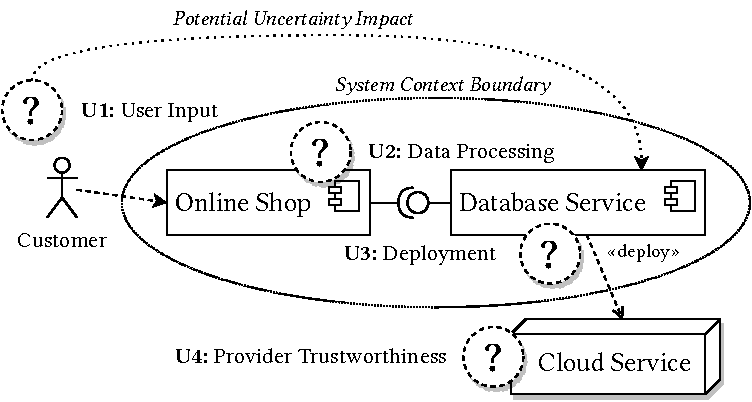
\includegraphics[width=0.8\textwidth]{figures/chapter5/onlineshop-context.pdf}
    \caption{Combined component and deployment diagram of the running example with annotated uncertainty sources, the system context boundary, and the impact of the user input uncertainty source.}
    \label{fig:classification:example}
\end{figure}


\subsection{Existing Notions of Uncertainty}

Multiple definitions of uncertainty exist, see \autoref{sec:foundations:uncertainty}.
Regarding software-architectural uncertainty, we consider two major points of view.
First, the concept of uncertainty stemming from the research community of \acp{SAS} \cite{weyns_towards_2023,weyns_introduction_2020}.
Here, uncertainty is often referred to as unanticipated change, fuzziness, noise, or incomplete knowledge \cite{weyns_towards_2023} and located within the system context or environment \cite{weyns_introduction_2020}.
Uncertainty is seen as a challenge which has to be considered within the system design and \enquote{engineering software-intensive systems that can handle uncertainty is complex} \cite{weyns_introduction_2020}.
Second, from a software engineering point of view, the \emph{cone of uncertainty} describes the inherent phenomenon of the lack of knowledge about a software system in early development phases \cite{mcconnell_software_1998}.
Here, uncertainty is constituted as part of every software project and is reduced over time, e.g., by making design decisions like \acp{ADD}.
In our running example, the user input (\U{1}) as human in the loop and the provider trustworthiness (\U{4}) as uncertain environment represent uncertainty sources known from \acp{SAS}.
Opposite to this, the data processing (\U{2}) and the deployment (\U{3}) represent design decisions that would reduce the \emph{cone of uncertainty}.
Regarding software-architectural uncertainty, we do not distinguish between these two perspectives, as both are relevant regarding confidentiality.
As long as we can represent the uncertainty sources in architectural models and analyze their impact, we can asses their effect on confidentiality.

When dealing with software-architectural uncertainty, considering \acp{ADD} helps to structure the design process.
At the beginning of this process, much is yet unknown or imprecise and \acp{ADD} are made under assumptions \cite{mcconnell_software_1998}, e.g., that the provider is trustworthy in Uncertainty \U{4}.
Making this uncertainty explicit can help to mark decisions as challenged \cite{kruchten_ontology_2004} and consider backtracking\footnote{A couple of years ago, I had the possibility to discuss this very point with Philippe Kruchten. He stressed the importance and costs of backtracking due to false assumptions and design faults. This was another motivation to research the early identification and impact analysis of software-architectural uncertainty.}.
While some uncertainty only exists due to not yet decided \acp{ADD}, others cannot be reduced immediately \cite{perez-palacin_uncertainties_2014}, e.g., Uncertainty \U{1} regarding the user input.
Still, creating awareness of the uncertainty source can help refine the architecture and make more informed statements about confidentiality.
This way, uncertainty can be understood, modeled, analyzed, and---eventually---managed.

There are multiple relevant properties of \acp{ADD} that help in the mitigation of uncertainty.
The number of solutions of related \acp{ADD} \cite{jansen_software_2005} can help to estimate whether the uncertainty can already be fully reduced at design time, e.g., by design space exploration \cite{esfahani_guidearch_2013,koziolek_peropteryx_2011}.
We distinguish between closed sets that could at least partially be analyzed and open sets with a potentially infinite number of solutions or configurations.
In our example, Uncertainty \U{3} relates to the \ac{ADD} of the deployment of the \emph{Database Service} and represents a closed set.
But even with a closed set of alternatives, one cannot guarantee that a given \ac{ADD} might not be challenged in the future \cite{kruchten_ontology_2004} due to changes in requirements or the system's execution context.
Thus, when speaking about decisions under uncertainty, considering the probability, possibility and costs of revisions can help to quantify the risk.
This awareness also helps in the prioritization of \acp{ADD} and deciding whether existing mitigation is sufficient.

However, only considering \acp{ADD} to understand the impact of uncertainty is not enough because uncertainty might not be directly connected to a single decision, e.g., to resolve Uncertainty \U{4}.
We argue to also consider which architectural elements are affected, rather than only considering this transitively via the impact of \acp{ADD}.
This does help in understanding the consequences of uncertain influences regarding confidentiality and also helps to connect these to architectural analyses to identify confidentiality violations.

\finding{%
Different notions of uncertainty exist, e.g., the \emph{cone of uncertainty} or uncertainty in \acfp{SAS}.
We do not limit software-architectural uncertainty to one of these notions, as all of these uncertainties can affect confidentiality.
Regarding the software architecture, considering \acfp{ADD} helps for early assessment and prioritization.}


\subsection{Investigating Existing Uncertainty Classifications}%
\label{sec:classification:investigating}

Based on our understanding of the relation of uncertainty, software architecture, and confidentiality presented in the previous section, we investigate existing uncertainty classifications stemming from related work.
Hereby, we address Problem \PR{1}{2} regarding the need for a classification tailored to confidentiality.
As discussed previously and also in \autoref{sec:foundations:uncertainty}, there are many types, notions, and dimensions of uncertainty.
In the following, we follow a top-down approach by discussing shortcomings of classifications and taxonomies while focusing on confidentiality.

We gathered and assessed categories, i.e., dimensions, or characteristics, and options, i.e., entries of a category in \autoref{sec:foundations:uncertainty}.
Here, the first category was the \emph{location} of uncertainty, see \autoref{table:foundations:sources:locationlevel}.
Although this category is used in many taxonomies \cite{bures_capturing_2020,mahdavi-hezavehi_classification_2017,perez-palacin_uncertainties_2014,walker_defining_2003,troya_uncertainty_2021,PSUM}, is has several shortcomings. 
There is no common distinction between the source and the impact location of uncertainty.
Also, there is no common understanding of the term \emph{model} as the taxonomies originate from different research areas.
This impedes the common understanding of uncertainty regarding confidentiality.
In the running example, Uncertainty \U{3} about the deployment could be classified as \emph{context}, \emph{model structural}, \emph{model technical}, and \emph{belief uncertainty}.
Such ambiguity can invalidate the purpose of a classification.
The second category was the \emph{level} of uncertainty, see \autoref{table:foundations:sources:locationlevel}. 
In the running example, all uncertainty sources represent known unknowns, i.e., first-order uncertainty, because we are aware of the sources and can annotate them in the architectural model.
However, the concrete representation might be different, e.g., using scenarios to describe the deployment of Uncertainty \U{3}.
As discussed previously, we find distinguishing between a \emph{known} and \emph{unknown} uncertainty to be not expedient as it only depends on the viewpoint of the software architects whether they are aware of the uncertainty source.

The next three categories are the \emph{nature}, \emph{manageability}, and the \emph{resolution time}, see \autoref{table:foundations:sources:naturemanagetime}.
In our running example, the uncertainty sources in the software system, i.e., Uncertainty \U{2} about the data processing and Uncertainty \U{3} about the deployment, represent epistemic uncertainty.
The uncertainty sources in the system context, i.e., Uncertainty \U{1} about the user input and Uncertainty \U{4} about the provider trustworthiness can be classified as epistemic or aleatory, depending on the point of view.
This shows again the ambiguity of this category.
All uncertainties in the running example can be described using scenarios and resolved between design and run time.

The last categories are the \emph{impact on quality} of uncertainty and the \emph{relationships} between uncertainties.
To focus analysis capabilities, software architects must know about potential impacts and their severity.
Although we focus on confidentiality, the analysis of multiple properties is possible, e.g., by using software architecture evaluation approaches under uncertainty \cite{sobhy_evaluation_2021}.
In the running example, all four uncertainty sources can have an impact on confidentiality.
Uncertainty relationships can cause hard-to-find problems regarding quality properties \cite{camara_addressing_2022}.
However, they often require further analysis based on the software system under study \cite{camara_uncertainty_2024}.
In the running example, there is such a relationship between Uncertainty \U{3} about the deployment and Uncertainty \U{4} about the provider's trustworthiness.
The latter only affects the confidentiality of the software system if the cloud provider is chosen in the first place.
As described above, such uncertainty interactions have to be further analyzed \cite{camara_uncertainty_2024}, and cannot be generally described using a classification.

\finding{The literature comprises many classifications and taxonomies of uncertainty that propose categories like location, level, or nature.
Despite being mostly relevant regarding confidentiality, they use varying terminology, contain ambiguity, and do not focus on uncertainty sources.
Thus, they have to be adapted to classify software-architectural uncertainty sources.}





\section{Classification of Uncertainty Regarding Confidentiality}%
\label{sec:classification:classification}

Based on the categories and options we identified in existing classifications of uncertainty, we define a novel classification scheme of uncertainty regarding confidentiality.
This allows us to build on existing knowledge from the domain of \acp{SAS} while aligning the classification to software-architectural uncertainty and confidentiality.
Additionally, we focus on uncertainty \emph{sources} as the primary concern regarding identification and early mitigation \cite{ramirez_taxonomy_2012,perez-palacin_uncertainties_2014}, see \autoref{sec:classification:relation}.
This addresses our second Problem \PR{1}{2} regarding the need for a classification tailored to confidentiality.

Our classification scheme consists of 8 categories with a total of 27 options and is shown in the tables \ref{table:classification:classification:location} -- \ref{table:classification:classification:severityoftheimpact}.
The categories are based on taxonomies of uncertainty \cite{bures_capturing_2020,esfahani_uncertainty_2013,mahdavi-hezavehi_classification_2017,perez-palacin_uncertainties_2014,ramirez_taxonomy_2012,walker_defining_2003,PSUM}, related work on \acp{ADD} \cite{jansen_software_2005,kruchten_ontology_2004} and \acp{ADL} like the \ac{PCM} \cite{reussner_modeling_2016}.
A category-based classification helps to group uncertainties and identify similar characteristics and mitigation approaches.
Once classified, the information can be reused across different software architectures.
To create this classification, we assessed and adapted existing categories and combined or refined their options, see \autoref{sec:classification:investigating}.
We repeated this process until each category fulfilled its purpose, i.e., being able to describe and partition uncertainty sources with respect to confidentiality in software architectures.

In this work, we focus on confidentiality requirements during the design time. 
Thus, the categories should be interpreted from an architectural point of view, e.g., while modeling a software system. 
In the following, we explain each category in detail.
We provide information about the rationale and possible benefits of applying each category.
We also define whether the options are unordered, i.e., \emph{nominal}, or ordered without defined distance, i.e., \emph{ordinal}.
Last, we specify if the gained knowledge by classification can be reused.
Here, a category can be specific for the uncertainty source and thus \emph{system-independent}, or specific for the software architecture under investigation and thus \emph{system-specific}.
This also concerns the question of whether the specific classification of a source of uncertainty is \emph{immutable} and does not change after the identification or \emph{mutable} and can be changed if more information is obtained during modeling and analysis.


\subsection{Classification Category: Location}

\begin{table}
    \begin{tabularx}{\textwidth}{lX}
        \toprule
        \tableheading{Location}{Describes where an uncertainty manifests itself within the architecture\\and which view or concern of the software architecture is primarily applicable.\\ \classificationtags{System-Independent}{Nominal}{Immutable}}
        \midrule
        \tableentry{System Structure}{The uncertainty is related to the structure of the software system and becomes visible in structural views, e.g., component diagrams, or class diagrams.}
        \tableentry{System Behavior}{The uncertainty is related to the behavior of the software system and becomes visible in behavioral views, e.g., activity diagrams, or sequence diagrams.}
        \tableentry{System Environment}{The uncertainty is related to the environmental context of the software system and becomes visible when considering external factors, e.g., in deployment diagrams.}
        \tableentry{System Input}{The uncertainty is related to the input to the software system and becomes visible when considering external interface specifications, or usage descriptions.}
        \bottomrule
    \end{tabularx}
    \caption{Uncertainty classification regarding confidentiality. Category: Location.}%
    \label{table:classification:classification:location}
\end{table}

The first category shown in \autoref{table:classification:classification:location} is concerned with the \emph{location} of the uncertainty source.
Previous taxonomies \cite{bures_capturing_2020,mahdavi-hezavehi_classification_2017,perez-palacin_uncertainties_2014,walker_defining_2003} already considered \enquote{where the uncertainty manifests itself within the model} \cite{perez-palacin_uncertainties_2014} but did not explicitly relate to an \ac{ADL}.
Since the location of the source is one of the most important properties for design time modeling analysis, we define four locations as inspired by the viewpoints of the PCM \cite{reussner_modeling_2016}.
Compared to existing taxonomies, this enables more precise description and mitigation because we can model uncertainty and its relation to existing architecture elements.

The option \emph{system structure} describes uncertainty in components and their assembly, which becomes visible in structural views like component diagrams.
The option \emph{system behavior} describes uncertainty in the communication, e.g., related to the handling of data within a component or the communication between components.
The option \emph{system environment} describes uncertainty in the system's context including hardware resources and the external situation.
The option \emph{system input} describes uncertainty in inputs provided by external actors, e.g., people using the software system.
Note that we distinguish between the input, i.e., the user behavior, and the system behavior.
This is due to the special role---and rights---of humans with regard to confidentiality, e.g., due to legal requirements like the \ac{GDPR} \cite{council_of_european_union_regulation_2016}, and shall also help in collaboration with legal analysis \cite{boltz_model-based_2022}.
Because the location is defined on the level of an \ac{ADL} meta model, it is system-independent and immutable.
The category is nominal, as its options only represent viewpoints without applicable order.


\subsection{Classification Category: Architectural Element Type}

\begin{table}
    \begin{tabularx}{\textwidth}{lX}
        \toprule
        \tableheading{Architectural Element Type}{Describes the type or class of elements to which an\\uncertainty can be assigned when considering its impact on a software system's\\confidentiality. \classificationtags{System-Independent}{Nominal}{Immutable}}
        \midrule
        \tableentry{Component}{The uncertainty is assignable to software components. This represents the nodes of a software system.}
        \tableentry{Connector}{The uncertainty is assignable to wires between components, or their communication. This represents the edges between the nodes of a system.}
        \tableentry{Interface}{The uncertainty is assignable to interfaces of components. This represents the contact point of nodes and edges in a software system.}
        \tableentry{External}{The uncertainty is assignable to external resources or their properties. This represents annotating the nodes of a software system.}
        \tableentry{Behavior}{The uncertainty is assignable to behavior descriptions. This represents specifying the behavior of nodes within a software system.}
        \bottomrule
    \end{tabularx}
    \caption{Uncertainty classification regarding confidentiality. Category: Architectural Element Type.}%
    \label{table:classification:classification:architecturalelementtype}
\end{table}

\autoref{table:classification:classification:architecturalelementtype} shows the second category \emph{Architecture Element Type}.
While the \emph{Location} is on the abstraction of the viewpoint (e.g., structure, or behavior), the \emph{Architecture Element Type} describes the concrete elements where the uncertainty arises.
Similarly to the previous category, the options are inspired by software architecture element types known from \acp{ADL} like the \ac{PCM}.
We consider this to be the central category for further modeling and analysis of uncertainty, as it specifies a starting point to consider the effect of an uncertainty source.
Compared to existing classifications, we provide five concrete options rather than only speaking of uncertainty within the model \cite{perez-palacin_uncertainties_2014}.
The need for such precision is supported by more recent approaches to classifying and propagating uncertainty \cite{acosta_uncertainty_2022,camara_uncertainty_2024} and also in the recent \ac{PSUM} standard \cite{PSUM}.
By understanding which elements and viewpoints are affected, software architects can assess responsibilities and evaluate mitigation methods.

The option \emph{component} describes uncertainty assignable to software components, e.g., related to their allocation or other component-wide decisions or properties.
The option \emph{connector} describes uncertainty assignable to, e.g., wires between components and thus communication and its properties.
The option \emph{interface} describes uncertainty assignable to interfaces, e.g., signatures, parameters, and return values.
The option \emph{external} describes uncertainty assignable to hardware resources, e.g., servers, and external actors like users of the system.
Note that we renamed this category compared to the original publication \cite{hahner_classification_2023} to take into account that users also represent external entities.
The option \emph{behavior} describes uncertainty assignable to behavior descriptions, e.g., algorithms, user behavior and input, data processing, and persistence.
This option also helps to underline the difference between \emph{Architecture Element Type} and \emph{Location}: Although behavior descriptions of users and the software system may be similar, the viewpoints of \emph{System Behavior} and \emph{System Input} are different.
Both categories are orthogonal and cannot be replaced by each other.
The category is immutable and system-independent and can thus be reused across architectural models.
The category is nominal as there is no order between location or element types.


\subsection{Classification Category: Type}

\begin{table}
    \begin{tabularx}{\textwidth}{lX}
        \toprule
        \tableheading{Type}{Describes how much is known about uncertainty and how it is described\\on a scale from only being aware to having precise knowledge. This may change\\with growing knowledge. \classificationtags{System-Specific}{Ordinal}{Mutable}}
        \midrule
        \tableentry{Statistical Uncertainty}{The uncertainty can be described with statistical means, e.g., related to the probability of certain outcomes.}
        \tableentry{Scenario Uncertainty}{The uncertainty can be described with distinct scenarios but there is a lack of knowledge to apply statistical means.}
        \tableentry{Recognized Ignorance}{There is awareness of the uncertainty but no knowledge about potential scenarios or lack of a description strategy. This is the most general form of an identfied uncertainty source.}
        \bottomrule
    \end{tabularx}
    \caption{Uncertainty classification regarding confidentiality. Category: Type.}%
    \label{table:classification:classification:type}
\end{table}

The third category is called \emph{Type} and describes how much is known about the uncertain influence as shown in \autoref{table:classification:classification:type}.
Other taxonomies \cite{bures_capturing_2020,perez-palacin_uncertainties_2014} only specify this in terms of levels on a scale from knowledge to ignorance \cite{armour_five_2000}, which is too imprecise to classify uncertainty for later mitigation.
With the \emph{Type}, we describe how much is known about the uncertainty, based on the definitions by Walker et al. \cite{walker_defining_2003}.
As discussed previously, we do distinguish between known or unknown unknowns as this depends on the viewpoint of the software architect and not the classified uncertainty source.

\emph{Statistical} uncertainty implies that the uncertainty is describable with statistical means, e.g., stochastic expressions, or probability distributions.
\emph{Scenario} uncertainty implies that the uncertainty can be represented with distinct scenarios depending on the uncertain outcome but without statistical means.
\emph{Recognized ignorance} only implies awareness of uncertainty sources, without scenario-based or statistical means to describe their form. 
These options can be ordered depending on the amount of knowledge and thus are ordinal.
Having statistical information enables more precise analysis results than just knowing scenarios---which is still better than simple awareness.
The category is system-specific and mutable.
During the software design and realization, more information may be gained, enabling a more precise description of the uncertainty, e.g., because more statistical information is collected or some scenarios can be excluded.


\subsection{Classification Category: Manageability}

\begin{table}
    \begin{tabularx}{\textwidth}{lX}
        \toprule
        \tableheading{Manageability}{Describes to which extent the uncertainty can be managed, reduced,\\or mitigated. This only provides a first estimate and may change with growing\\knowledge. \classificationtags{System-Specific}{Ordinal}{Mutable}}
        \midrule
        \tableentry{Fully Reducible}{The uncertainty can be fully resolved with appropriate means that mitigate its potential impact.}
        \tableentry{Partially Reducible}{The uncertainty is at least partially reducible which reduces the potential impact severity or limits critical outcomes by appropriate mitigation techniques.}
        \tableentry{Irreducible}{The uncertainty cannot be further reduced as there is no reasonable way to achieve the required knowledge at this point in time.}
        \bottomrule
    \end{tabularx}
    \caption{Uncertainty classification regarding confidentiality. Category: Manageability.}%
    \label{table:classification:classification:manageability}
\end{table}

The fourth category shown in \autoref{table:classification:classification:manageability} covers the \emph{manageability} of uncertainty.
\emph{Manageability} states whether we can control or reduce the impact of the uncertainty at design time or are only aware of it \cite{esfahani_uncertainty_2013}.
Early identification of potential threats to security-related properties like confidentiality is also required by \emph{Data Protection by Design} \cite[Art.~25]{council_of_european_union_regulation_2016}. 
We do not consider the nature of the uncertainty \cite{walker_defining_2003} because the manageability is closer to the uncertainty's impact on the software system \cite{esfahani_uncertainty_2013}.
Representing the manageability on a scale from reducibility to irreducibility is also supported by the \ac{PSUM} standard \cite{PSUM}.

\emph{Fully reducible} uncertainty can be fully reduced by taking appropriate actions, e.g., an \ac{ADD} at design time, or comprehensive simulation. This can include \enquote{collecting additional information until achieving full certainty} \cite{PSUM}.
\emph{Partially reducible} implies that full certainty cannot be reached.
Nevertheless, the uncertainty can be reduced by collecting more information, or by applying scenario-based mitigation strategies, or system-wide constraints and policies.
\emph{Irreducible} uncertainty cannot be further reduced, e.g., due to its aleatory nature \cite{perez-palacin_uncertainties_2014,PSUM}.
Similar to the type category, this category is ordinal because the options can be ordered.
The classification depends on the architecture under investigation and the current knowledge.
Thus, this option is system-specific and mutable.
However, many uncertainty types tend to be categorized similarly across architectures.


\subsection{Classification Category: Resolution Time}

\begin{table}
    \begin{tabularx}{\textwidth}{lX}
        \toprule
        \tableheading{Resolution Time}{Describes the rough time span in the development process where\\the uncertainty is usually expected to be fully resolved.\\ \classificationtags{System-Independent}{Ordinal}{Immutable}}
        \midrule
        \tableentry{Requirements Time}{The uncertainty is expected to be resolved as soon as the requirements are defined.}
        \tableentry{Design Time}{The uncertainty is expected to be resolved as soon as the software system is designed.}
        \tableentry{Realization Time}{The uncertainty is expected to be resolved as soon as the software system or parts of it are implemented and deployed.}
        \tableentry{Runtime}{The uncertainty is expected to be resolved as knowledge is gained from testing and system operations, or not at all.}
        \bottomrule
    \end{tabularx}
    \caption{Uncertainty classification regarding confidentiality. Category: Resolution Time.}%
    \label{table:classification:classification:resolutiontime}
\end{table}

The \emph{Resolution Time} shown in \autoref{table:classification:classification:resolutiontime} is based on the phases of software development and can help to narrow down sources and responsibilities.
Since we focus on the impact of uncertainty on confidentiality, we consider the expected full resolution time rather than the emerging time \cite{hezavehi_uncertainty_2021,perez-palacin_uncertainties_2014,ramirez_taxonomy_2012,troya_uncertainty_2021}.
Also, we only include phases that are relevant from the point of view of design time modeling and analysis.

\emph{Requirements time} implies that the uncertainty resolves as soon as requirements are defined, e.g., related to confidentiality requirements or security policies.
\emph{Design time} implies that the uncertainty resolves as soon as the system is designed, e.g., because the uncertainty is related to \acp{ADD}, the system structure, or software components.
\emph{Realization time} implies that the uncertainty resolves as the system or parts of it are implemented and deployed.
Here, we combine implementation and deployment as a distinction is not expedient from an architectural point of view.
\emph{Runtime} implies that the uncertainty resolves at runtime, e.g., because knowledge is gained from testing or dynamic analysis like monitoring or profiling.
This category depends on the uncertainty source and not on the system under study and is thus system-independent and immutable.
It is ordinal because we can order the options along the phases of software development from requirements to runtime.


\subsection{Classification Category: Reducible by ADD}

\begin{table}
    \begin{tabularx}{\textwidth}{lX}
        \toprule
        \tableheading{Reducible by ADD}{Describes whether the uncertainty is resolvable or treatable by\\an architectural design decision, i.e., a decision that specifies or restricts a software\\systems's structure or behavior, thereby limiting the design space.\\ \classificationtags{System-Independent}{Nominal}{Immutable}}
        \midrule
        \tableentry{Yes}{The uncertainty can be reduced by making an architectural design decision.}
        \tableentry{No}{The uncertainty is not resolvable by taking an architectural design decision.}
        \bottomrule
    \end{tabularx}
    \caption{Uncertainty classification regarding confidentiality. Category: Reducible by ADD.}%
    \label{table:classification:classification:reduciblebyadd}
\end{table}

\autoref{table:classification:classification:reduciblebyadd} shows the category \emph{Reducible by ADD} that specifies whether the uncertainty source can at least be partially mitigated by a design decision on architectural abstraction, i.e., an \ac{ADD}.
Making the connection between \acp{ADD} and uncertainty explicit \cite{lytra_supporting_2013} helps to prioritize, e.g., check whether multiple or critical uncertainty sources can be tackled by a single decision.
\acp{ADD} are seen as crucial aspect of software architecture \cite{jansen_software_2005,kruchten_ontology_2004,alexeeva_design_2016}. 

The option \emph{Yes} describes uncertainty which can be addressed on architectural abstraction by making appropriate decisions, i.e., by designing the system in a way that the impact of the uncertainty is (partially) mitigated
This implies that the uncertainty can---and probably should---be addressed in the architectural design and falls into the \emph{cone of uncertainty} \cite{mcconnell_software_1998}.
The option \emph{No} describes uncertainty that is not resolvable or treatable by taking an \ac{ADD}, e.g., because the uncertainty is outside the scope of the designed software system, or cannot be properly addressed within the design process, e.g., due the behavior of a third-party.
An uncertainty that is not resolvable by an \ac{ADD} does not imply a resolution later than design time.
The uncertainty could also exist due to a lack of knowledge or could be addressed on a lower level than architectural abstraction---but not by an \ac{ADD}.
Both categories are orthogonal.
Reducibility is nominal, system-independent and immutable.


\subsection{Classification Category: Impact on Confidentiality}

\begin{table}
    \begin{tabularx}{\textwidth}{lX}
        \toprule
        \tableheading{Impact on Confidentiality}{Describes the impact on confidentiality requirements.\\Initially, this only provides a first, system-independent estimate.\\ \classificationtags{System-Specific}{Ordinal}{Mutable}}
        \midrule
        \tableentry{Direct}{The uncertainty has a direct impact on the software system's confidentiality.}
        \tableentry{Indirect}{The uncertainty only has an indirect impact on the software's confidentiality that usually relies on other uncertainties or other contextual factors.}
        \tableentry{None}{The uncertainty is expected to have no impact on confidentiality at all.}
        \bottomrule
    \end{tabularx}
    \caption{Uncertainty classification regarding confidentiality. Category: Impact on Confidentiality.}%
    \label{table:classification:classification:impactonconfidentiality}
\end{table}

The last two categories are used to quantify the impact of uncertainty on confidentiality requirements.
\autoref{table:classification:classification:impactonconfidentiality} shows the category \emph{Impact on Confidentiality}.
It represents a first estimate on whether the uncertainty can directly impact confidentiality or requires additional conditions to result in confidentiality violations.

The option \emph{Direct} describes uncertainty with a direct impact that can void confidentiality even without taking other factors, decisions, or uncertainties into account, e.g., by directly affecting input, processing, or storage of sensitive data like user data.
The option \emph{Indirect} describes uncertainty that is related to \acp{ADD}, security measures, or other uncertainty sources.
The option \emph{None} describes uncertainty without impact on confidentiality, e.g., if it is related to handling non-sensitive data or well-secured system parts or because the uncertainty has no effect on any data processing at all, e.g., related to the color of a button.
Note that this category only describes the type of impact but not its severity.
An indirect impact can be as severe as a direct impact but is potentially even harder to identify.
This category only provides a first, mutable estimate and is highly system-specific.
We consider the options to be ordinal as they can be sorted from direct to no impact.


\subsection{Classification Category: Severity of the Impact}

\begin{table}
    \begin{tabularx}{\textwidth}{lX}
        \toprule
        \tableheading{Severity of the Impact}{Describes the severity if the uncertainty is not mitigated.\\Initially, this only provides a first, system-independent estimate.\\ \classificationtags{System-Specific}{Ordinal}{Mutable}}
        \midrule
        \tableentry{High}{The uncertainty can cause a total loss of confidentiality, e.g. due to a data breach.}
        \tableentry{Low}{The uncertainty can cause information leaks, but the damage is limited.}
        \tableentry{None}{The uncertainty is expected to cause no loss of confidentiality at all.}
        \bottomrule
    \end{tabularx}
    \caption{Uncertainty classification regarding confidentiality. Category: Severity of the Impact.}%
    \label{table:classification:classification:severityoftheimpact}
\end{table}

To prioritize uncertainty with a potentially critical impact, we combine the previously introduced impact type with its severity.
\autoref{table:classification:classification:severityoftheimpact} shows the last category of the classification that is named \emph{Severity of the Impact}.
This category is based on the confidentiality impact metrics of the open industry standard \acf{CVSS} \cite{CVSS}.
We reuse the definition as it is broadly used, and known by security experts.

The option \emph{High} refers to uncertainty that can cause the total loss of confidential data or access to restricted information.
This can be the case because the uncertainty is either related to highly sensitive data like certificates, encryption keys, or an admin password or because the uncertainty is related to central security measures like input validation and sanitization.
The option \emph{Low} refers to uncertainty that could cause the loss of restricted information, but the damage is limited, e.g., because the input validation only has limited effects due to insufficient security policies.
The option \emph{No} refers to uncertainty where no loss of confidentiality is expected at all, e.g., because the uncertainty is related to parts of a software system that do not deal with sensitive information.
As stated in the previous category, there is no clear dependency between an impact's type and its severity.
Only uncertainty sources that have no impact on confidentiality at all are also expected to have no severity.
Other than that, any combination of high or low, and direct or indirect can happen. 
This category as well provides a first, mutable estimate that is system-specific.
Nevertheless, both categories help to estimate the potential impact and plan further steps toward analyzing the uncertainty. 
The knowledge gained by this classification can help in clustering and prioritizing uncertainty and related \acp{ADD}.
This category is ordinal.


\subsection{Building on the Uncertainty Classification}

In sum, our classification provides eight categories that do not classify uncertainty in isolation but also relate the uncertainty sources to software architecture and confidentiality, as discussed in \autoref{sec:classification:relation}.
These categories help in the early understanding of uncertainty sources and serve the discussion of software architects and security experts.
We split the categories into system-independent and system-specific.
System-specific categories are always mutable, as the knowledge about the uncertainty source can change over time.

\finding{Uncertainty classifications are a well-suited entry point to understanding uncertainty sources.
However, classification can change over time when more knowledge is gained or the system or environment changes.
Some categories of the classification depend on the architecture under study.
Still, many uncertainty sources tend to be categorized similarly across architectures.}

This classification represents the baseline for further modeling and analysis activities, as outlined in \autoref{sec:overview:procedure}.
Many categories help in the early assessment of the criticality of an uncertainty source, even without systematically analyzing the software architecture.
However, to gain detailed insights on the impact of uncertainty and to identify confidentiality violations, architecture-based analysis is expedient.
Here, we benefit from the category \emph{Architectural Element Type}, which relates uncertainty sources to concrete element types of software architectures and can be used to extend existing \acp{ADL} like the \ac{PCM}.

\finding{Centering an uncertainty classification around the location of the uncertainty source simplifies the later modeling, analysis, and mitigation.
Thus, we see the category \emph{Architectural Element Type} and its options \emph{Component}, \emph{Connector}, \emph{Interface}, \emph{External}, and \emph{Behavior} as central dimension of our classification.}

This finding is supported by comparable approaches \cite{acosta_uncertainty_2022,camara_uncertainty_2024} that analyze the impact of uncertainty.
\textcite{acosta_uncertainty_2022} define the category \emph{Locus} that describes the location of uncertainty within the model and serves as starting point of uncertainty propagation.
Due to the importance of this category, we will use it throughout the remainder of this thesis and refer to it directly, e.g., by speaking of \emph{Component} uncertainty, \emph{Behavior} uncertainty, or \emph{External} uncertainty.





\section{Applying the Classification to the Running Example}%
\label{sec:classification:runningexample}

We illustrate the classification introduced in the previous section by applying it to the running example from \autoref{ch:runningexample}.
The running example, which shows a simplified online shop, comprises four uncertainties: The user input, data processing within the \emph{Online Shop} component, the deployment of the \emph{Database Service}, and the provider trustworthiness of the \emph{Cloud Service} resource.
In the following, we present one possible classification using the aforementioned classification scheme.
While some categories like the location are system-independent, others like the severity regarding confidentiality are system-specific and are based on our interpretation of the running example.
We provide our reasoning and also explain alternative classifications.
All classified uncertainty sources are part of our data set \cite{dataset}.
Additionally, they are listed in \arcen with the proposed classification\footnote{At the time of writing, \arcen is online available here: \url{https://arc3n.abunai.dev/}. Currently, the uncertainty sources of the running example \U{1} -- \U{4} are listed as \href{https://arc3n.abunai.dev/uncertainty/52}{\#52}, \href{https://arc3n.abunai.dev/uncertainty/35}{\#35}, \href{https://arc3n.abunai.dev/uncertainty/59}{\#59}, and \href{https://arc3n.abunai.dev/uncertainty/48}{\#48}.}.


\begin{table}
    \centering
    \begin{tabular}{lll}
        \toprule
        Category                        & \U{1}: User Input   & \U{2}: Data Processing \\
        \midrule
        Location                        & System Input              & System Behavior \\
        Architectural Element Type\;    & Connector                 & Behavior \\
        Type                            & Scenario Uncertainty\;    & Scenario Uncertainty \\
        Manageability                   & Partially Reducible       & Fully Reducible \\
        Resolution Time                 & Runtime                   & Design Time \\
        Reducible by ADD                & Yes                       & Yes \\
        Impact on Confidentiality       & Indirect                  & Direct \\
        Severity of the Impact          & High                      & High \\
        \bottomrule
    \end{tabular}
    \caption{Exemplary classification of the uncertainty sources U1 and U2 in the running example.}%
    \label{table:classification:example:one}
\end{table}

\autoref{table:classification:example:one} shows our classification of the first two uncertainty sources, i.e., the user input (\U{1}) and the data processing (\U{2}).
The Uncertainty \U{1} about the user input is located in the system input and can be annotated at a connector.
We annotate the uncertainty to a connector instead of a behavior description because it relates to the question of how the user communicates with the system.
In our discussion in \autoref{sec:runningexample:uncertainty}, we enumerated scenarios like normal or malicious behavior, thus we already reached the knowledge of scenario uncertainty.
With mitigation strategies like proper input validation, we can at least partially reduce the uncertainty---more optimistic experts could even argue for full reducibility.
The uncertainty persists until run time when actual humans use the system under study.
Until then, it is reducible by appropriate design decisions like the aforementioned input validation.
The input on confidentiality in our example is indirect as it depends on the data processing, and thus, it depends on Uncertainty \U{2} whether confidentiality could be violated.
If we do not have any means of input validation, the impact could be direct.
We classify the severity as high because confidentiality cannot be guaranteed under this uncertainty.

The Uncertainty \U{2} about the data processing is located in the system behavior and can be represented in a behavior description.
Similarly to Uncertainty \U{1}, we already provided scenarios in \autoref{sec:runningexample:uncertainty}, thus, it represents scenario uncertainty.
The uncertainty about the data processing is an uncertainty due to an open \ac{ADD} as described by the \emph{cone of uncertainty} \cite{mcconnell_software_1998}.
Thus, it is fully reducible already at design time.
We classify the impact on confidentiality as direct and high, because improper processing directly and severely affects the confidentiality, e.g., because of missing validation or encryption.


\begin{table}
    \centering
    \begin{tabular}{lll}
        \toprule
        Category                        & \U{3}: Deployment   & \U{4}: Provider Trustworthiness \\
        \midrule
        Location                        & System Structure          & System Environment \\
        Architectural Element Type\;    & Component                 & External \\
        Type                            & Scenario Uncertainty\;    & Scenario Uncertainty \\
        Manageability                   & Partially Reducible       & Partially Reducible \\
        Resolution Time                 & Realization Time          & Runtime \\
        Reducible by ADD                & Yes                       & Yes \\
        Impact on Confidentiality       & Direct                    & Indirect \\
        Severity of the Impact          & High                      & High \\
        \bottomrule
    \end{tabular}
    \caption{Exemplary classification of the uncertainty sources U3 and U4 in the running example.}%
    \label{table:classification:example:two}
\end{table}

\autoref{table:classification:example:two} shows our classification of the last two uncertainty sources, i.e., the deployment (\U{3}) and the provider trustworthiness (\U{4}). 
The Uncertainty \U{3} about the deployment is located in the system structure and can be annotated to a component that must be deployed.
In \autoref{sec:runningexample:architecture}, we describe two scenarios of this scenario uncertainty, i.e., deployment on premise, or in the cloud.
In our interpretation, this uncertainty is only partially reducible by a proper \ac{ADD} at design time as it resolves at realization time, i.e., when the component gets deployed after the architectural design of the software system.
In our running example, the impact on confidentiality is direct and high.
If the confidentiality requirements demand selected deployment locations due to legal requirements like the \ac{GDPR} \cite{council_of_european_union_regulation_2016}, any deviation causes a confidentiality violation.

The Uncertainty \U{4} about the trustworthiness of the cloud service provider is located in the system environment and classified as external uncertainty in the system's context, see \autoref{fig:classification:example}.
Although we cannot control the provider's behavior, we can describe scenarios, i.e., trustworthy or not trustworthy behavior.
With further knowledge or experience, experts could quantify the probability of these scenarios to reach statistical uncertainty, but in the running example, that is out of scope.
With proper \ac{ADD}, we can at least limit the impact of this uncertainty.
Thus, it is partially reducible.
In our running example, the impact on confidentiality is high but indirect.
The impact depends on the form of data processing (\U{2}) and also the deployment location (\U{3}).
Put simply, the cloud provider's trustworthiness does not affect the confidentiality if nothing is deployed in the cloud.

In sum, this illustration shows how our classification can be applied to better understand uncertainty sources.
Compared to other classifications, we focus on confidentiality and thus provide appropriate categories for this purpose\footnote{I discussed this question with Raffaela Mirandola, who co-authored one of the investigated classifications \cite{perez-palacin_uncertainties_2014}. We concluded that there is no such thing as a \emph{best} classification---only appropriate and less appropriate classifications for a specific \emph{purpose}.}.
Describing the uncertainty in these categories helps to better understand the relation and criticality of uncertainty sources.
In our running example, we can see the importance of proper data processing (\U{2}) even without applying automated architectural analyses.
We also see the importance of choosing the right deployment locations and can prioritize this \ac{ADD}.
Last, classifying uncertainty always has some level of interpretation.
Thus, the classification of similar uncertainty sources in other software systems could be different.
Moreover, our classification could change at a later stage, e.g., when enough knowledge about the uncertainty sources and the probability of certain scenarios is gained for statistical analysis.





\section{Representing Uncertainty in Data Flow Diagrams}%
\label{sec:classification:dfd}

Analyzing confidentiality with \acfp{DFD} \cite{tuma_flaws_2019,schneider_automatic_2023,seifermann_detecting_2022} has been proposed because \enquote{problems tend to follow the data flow, not the control flow} \cite{shostack_threat_2014}.
Thus, Problem \PR{1}{3} is concerned with the representation of uncertainty in \acp{DFD}.
We address this by connecting \acp{DFD} to the \emph{Architectural Element Type} category of our classification.
As concluded previously in \autoref{sec:classification:classification}, this category is crucial for modeling and analyzing uncertainty on architectural abstraction.
This applies to \acp{ADL} like the \ac{PCM} \cite{reussner_modeling_2016} as well as to \acp{DFD}.
The following section builds on the foundations about \acp{DFD}, \acp{DAG}, and the unified modeling primitives \cite{seifermann_unified_2021} presented in \autoref{sec:foundations:dfd}.


\subsection{Mapping Uncertainty to Data Flow Diagrams}

\acp{DFD} consist of processes, data flows, files, data sources, and data sinks---put simply, different types of nodes and edges.
The unified modeling primitives \cite{seifermann_unified_2021} extend this notation and consist of nodes, pins, flows, behavior and labels with their assignments.
Nodes represent structural elements of software systems, e.g., processes, stores, or external entities.
Pins represent their interfaces and flows are used to connect multiple nodes through their pins.
Nodes have a defined behavior that assigns labels, e.g., based on labels at the node's input pins, constants, logical expressions or a combination of the above.
In our running example presented in \autoref{ch:runningexample}, we can represent the data processing of the \emph{Online Shop} component as a process node.
The node has one input pin for the incoming data flow from the user and one output pin for the outgoing, processed data flowing to the \emph{Database Service}.
The deployment of the \emph{Online Shop} component can be represented as a \emph{On Premise} label that is assigned to the process node.
Last, the behavior of the data processing node can be described using an assignment that assigns the label \emph{Encrypted} to all outgoing data to represent the encryption of all processed data.
For details on the unified modeling primitives of \acp{DFD}, see \autoref{sec:foundations:dfd} or the primary publication \cite{seifermann_unified_2021}.

In \autoref{table:classification:classification:architecturalelementtype}, we describe the category \emph{Architectural Element Type} which comprises the options component, connector, interface, external, and behavior.
Speaking in terms of nodes and edges, these options represent uncertainty, e.g., within a node in the case of component uncertainty, or at the contact point of a node and an edge in the case of interface uncertainty.
We build on this finding and the fact that \acp{DFD} are a viable representation of software architectures \cite{schneider_how_2024} to map the five uncertainty types to \acp{DFD}. 
\autoref{table:classification:mapping} shows the mapping of the five uncertainty types of the category \emph{Architectural Element Type} to the unified modeling primitives.


\begin{table}
    \centering
    \begin{tabular}{lll}
        \toprule
        Uncertainty Type \, & Modeling Primitives \, & Effect of the Uncertainty \\
        \midrule
        Component & Flow and node                           & Existence and use of nodes \\
        Connector & Flow and assignment                     & Existence and targets of flows \\
        Interface & Flow and pin                            & Existence and forms of pins \\
        External  & Label                                   & Existence of a node's labels \\
        Behavior  & Assignment                              & Existence of a node's assignments \\
        \bottomrule
    \end{tabular}
    \caption{Mapping of the five uncertainty types to the unified modeling primitives.}%
    \label{table:classification:mapping}
\end{table}

\emph{Component} uncertainty is assignable to software components that are represented by one or multiple nodes in a \ac{DFD}.
Thus, uncertainty regarding components affects the existence and use of nodes.
In our running example, Uncertainty \U{3} about the deployment can be represented as two alternative nodes where only one is in use.

\emph{Connector} uncertainty is assignable to the communication between entities, i.e., to the edges between nodes in a \ac{DFD}.
This affects the existence and targets of data flows.
Additionally, this uncertainty affects how and which data flows through an edge or data flow.
In our running example, we model Uncertainty \U{1} about the user input as connector uncertainty.
Here, different kinds of data, represented using assignments, can flow into the \emph{Online Shop} component, e.g., invalid or malicious data.

\emph{Interface} uncertainty is assignable to interfaces of components which are represented as pins in a \ac{DFD}.
This affects the existence and forms of pins.
Additionally, this uncertainty affects the data flows as an alternative interface can imply different processing which is represented as an alternative target of the data flow.
We do not model interface uncertainty in our running example; an example would be alternative signatures of the \emph{Database Service} which can be swapped and offer different data processing.

\emph{External} uncertainty represents annotations to nodes of software systems, e.g., components or resources, which are represented as nodes in \acp{DFD}.
This affects the assignment of labels to nodes.
In our running example, Uncertainty \U{4} about the provider's trustworthiness is an external uncertainty.
In a \ac{DFD}, the trustworthiness can be represented as a label that is or is not annotated to all nodes that represent the processes of the provider.

\emph{Behavior} uncertainty is assignable to behavior descriptions in architectural models which translate to behaviors and assignments following the unified modeling primitives \cite{seifermann_unified_2021}.
In our running example, Uncertainty \U{2} about the data processing can be represented as alternative behaviors, e.g., just forwarding the data or applying validation or encryption.
In sum, all uncertainty types are applicable to architectural models and also in \acp{DFD} that represent those models from the view of the data \cite{seifermann_data-driven_2019}.

Following the unified modeling primitives for \acp{DFD} by \textcite{seifermann_unified_2021}, we see how the \emph{Architectural Element Type} fits to the available elements types.
However, this is not obvious: The five options of this category, i.e., the five uncertainty types, were collected by investigating existing uncertainty classifications and \acp{ADL}.
Nevertheless, applying a bottom-up approach and starting with \acp{DFD} as underlying formalism yields the same five uncertainty types to represent uncertainty sources in all available element types.
The only exception is the element type \emph{Behavior}.
However, this type only acts as a container in the original definition of the unified modeling primitives \textcite{seifermann_unified_2021}.

\finding{The five uncertainty types described in the classification category \emph{Architectural Element Type} are derived from existing uncertainty classifications and \acfp{ADL} but also cover all elements of the unified modeling primitives for \acfp{DFD}. Although the representations are different, the five uncertainty types remain appropriate and applicable. Thus, the results of the bottom-up and top-down approaches match.}


\subsection{Mapping Uncertainty to Directed Acyclic Graphs}

In the following, we discuss how to include uncertainty as a first-class entity in \acp{DFD}, following the proposal of \textcite{garlan_software_2010}.
We simplify the representation of uncertainty by only considering \acp{DAG}.
\acp{DAG} can be used as simple formalism to represent \acp{DFD}, see \autoref{sec:foundations:dfd}.
Put simply, processes, files, data sources, and data sinks are denoted as vertices, and data flows are denoted as edges.
We go into more detail when we include uncertainty in architectural analyses---in this chapter, we remain at the conceptual level.

Looking at the affected modeling primitives in \autoref{table:classification:mapping}, we see that the former three uncertainty types affect flows while the latter two do not.
Speaking of \acp{DFD} in terms of vertices and edges of a \ac{DAG}, this is no coincidence.
Component uncertainty affects the choice of vertices and, therefore, also affects the edges to these vertices, and connector and interface uncertainty always affect the edges between vertices.
In contrast, external and behavior uncertainty directly affect the vertices, in terms of the unified modeling primitives, by affecting labels or assignments.
They do not affect edges\footnote{For you, dear reader, this may seem like an obvious or insignificant insight: Some uncertainties affect flows and others affect nodes. But, among others, this finding ultimately enabled us to create analyses that scale orders of magnitude better than the state of the art.}.

Based on this observation, we divide the five uncertainty types into two groups, which we call \emph{primary} and \emph{secondary} uncertainty.
\emph{Primary} uncertainty affects vertices and can directly be annotated to a vertex with an uncertainty source.
\emph{Secondary} uncertainty affects edges between vertices and can be annotated to an edge by adding alternative targets.
We use the terms primary uncertainty and secondary uncertainty to avoid ambiguity.
Direct or indirect uncertainty, structural uncertainty, higher-order uncertainty, and first-order or second-order uncertainty are already used in existing classifications \cite{perez-palacin_uncertainties_2014,walker_defining_2003,armour_five_2000}.

\begin{figure}
    \centering
    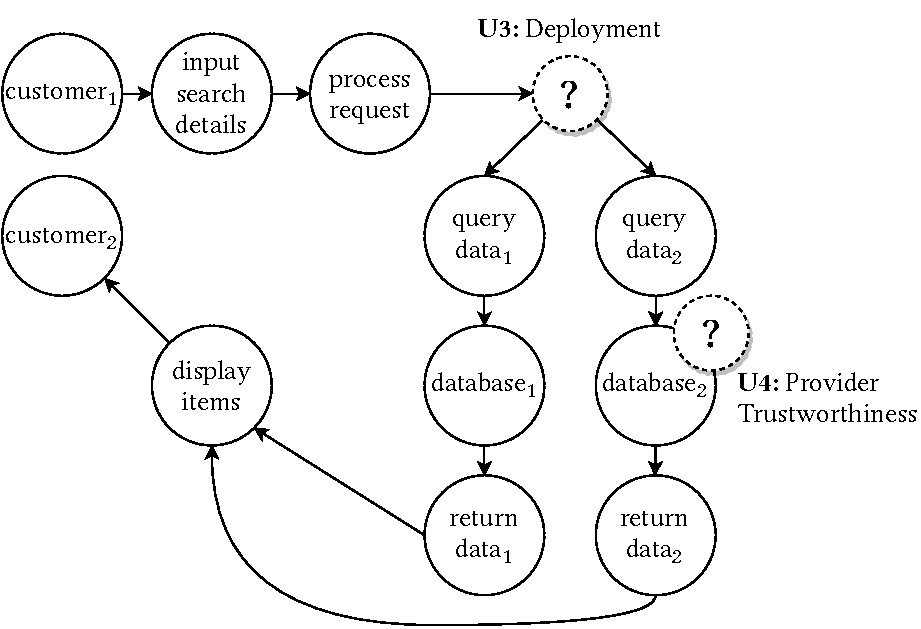
\includegraphics[width=0.85\textwidth]{figures/chapter5/onlineshop-dag.pdf}
    \caption{Data flow of the running example as \acf*{DAG} with annotated primary and secondary uncertainty, denoted by question marks.}
    \label{fig:classification:dag}
\end{figure}

\autoref{fig:classification:dag} shows the data flow of viewing available items from the running example, represented as \ac{DAG}.
We annotate the vertices and edges with primary and secondary uncertainty.
This example also illustrates how to transform a \ac{DFD} into a \ac{DAG}, as introduced in \autoref{sec:foundations:dfd}.
Cycles are replaced, e.g., the customer's sending and receiving activities are represented by separate vertices \cite{canfora_data_1992}.
The data flow of viewing available items is affected by two uncertainty sources: The uncertain deployment (\U{3}) and the provider's trustworthiness of the \emph{Cloud Service} (\U{4}).
The deployment (\U{3}) is classified as component uncertainty and thus falls into the group of \emph{secondary} uncertainty.
In this example, this affects the flow from the \emph{process request} vertex to the \emph{query data} vertices and all following vertices that represent the \emph{Database Service}.
The left flow from \emph{query data\textsubscript{1}} until \emph{return data\textsubscript{1}} represents the component being deployed on-premise, and the right flow represents the component being deployed in the cloud.
Here, we have to additionally consider the uncertainty about the provider's trustworthiness (\U{4}).
This uncertainty source is classified as external uncertainty and thus represents a \emph{primary} uncertainty.
For the sake of simplicity, we annotated this uncertainty only to the \emph{database\textsubscript{2}} vertex.

A \ac{DAG} $G = (V, E)$ consists of vertices $V$ and edges $E$.
Vertices affected by \emph{primary} uncertainty form a subset $V_{u} \subseteq V$.
We do not further restrict the size of $V_{u}$. 
The subset is empty if no primary uncertainty exists, but it can also contain every vertex of $V$.
In the running example, $V_{u} = \setted{\var{database_{2}}}$.
\emph{Secondary} uncertainty affects the edges of a \ac{DAG}.
Without limiting the generality, we can assume that the \ac{DAG} contains all known alternative scenarios, e.g., the deployment on-premise and in the cloud.
Then, each secondary uncertainty can be represented as a subset $E_{u_{i}} \subseteq E$.
All secondary uncertainties form a set $E_{u} = \setted{E_{u_{1}}, \dots, E_{u_{n}}}$ with size $\lvert E_{u} \rvert = n$.
Similarly, we do not further restrict its size but we require each edge to be contained at most once in a subset of a secondary uncertainty, i.e., $\forall e \in E, \forall i,j \in \setted{1, 2, \dots, n} : (e \in E_{u_{i}} \wedge i \neq j) \Rightarrow e \notin E_{u_{j}}$.
Otherwise, we would allow for the interference of secondary uncertainties.
In the running example, $E_{u_{1}} = \setted{\flow{process~request}{query~data_{1}}, \flow{process~request}{query~data_{2}}}$ and $E_{u} = \setted{E_{u_{1}}}$.

Already an example of this size demonstrates the benefits of including uncertainty as a first-class entity in the design \cite{garlan_software_2010}.
It helps to better understand the locations of uncertainty sources and even to investigate simple uncertainty interactions \cite{camara_uncertainty_2024}.
In this example, Uncertainty \U{4} is only relevant if the \emph{Cloud Service}, which is represented by the right data flow, is selected as deployment in Uncertainty \U{3}.
We consider this fact in the classification of the uncertainty sources in \autoref{sec:classification:runningexample}.
Here, we classify the impact of Uncertainty \U{3} as direct and the impact of Uncertainty \U{4} as indirect as it depends on another uncertainty, i.e., the Uncertainty \U{3}.
Representing uncertainty as primary and secondary uncertainty in \acp{DAG} visualizes such effects.
To this end, we actively manage a model with uncertainty instead of modifying the model to exclude uncertainty \cite{perez-palacin_dealing_2014}.

\finding{Including uncertainty sources as first-class entity in \acfp{DFD} simplifies their investigation, modeling, and analysis.
Even simple \ac{DFD} representations like \acfp{DAG} are sufficient to gain insights about the direct and indirect effects of uncertainty.
Here, we partition the five uncertainty types of the classification category \emph{Architectural Element Type} into two groups:
\emph{Primary} uncertainty directly affects vertices of \acp{DAG} while \emph{secondary} uncertainty affects edges between vertices.}





\section{Uncertainty Catalogs to Support the Identification}%
\label{sec:classification:identification}

Although classifying uncertainty is necessary to understand the differences in nature and type \cite{perez-palacin_uncertainties_2014}, it is not sufficient to enable the early identification of uncertainty sources.
Our classification shown in \autoref{sec:classification:classification} and also model-based confidentiality analyses require the uncertainty sources to be known to the software architect who conducts the assessment.
Uncertainty sources unknown to the architect, can neither be represented nor considered.
We motivated this \acf{UAP} already at the beginning of \autoref{ch:classification} and also in Problem \PR{1}{4}.

\begin{figure}
    \centering
    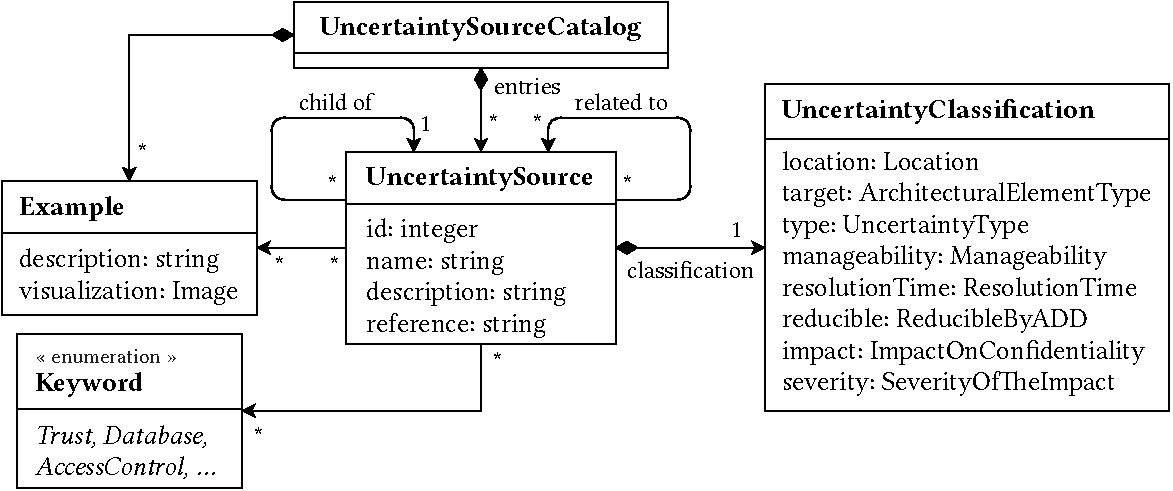
\includegraphics[width=\linewidth]{figures/chapter5/arc3n-metamodel.pdf}
    \caption[Simplified metamodel of the uncertainty source catalog.]{Simplified metamodel of the uncertainty source catalog. To simplify the illustration, we leave out all types of the UncertaintyClassification and refer to their comprehensive definition in \autoref{sec:classification:classification}.}
    \label{fig:classification:identification:metamodel}
\end{figure}

We propose a solution based on collecting and relating uncertainty sources and providing context information \cite{hahner_arcn_2024}.
\autoref{fig:classification:identification:metamodel} shows the metamodel of an \emph{Uncertainty Source Catalog}.
The \emph{Uncertainty Source Catalog} consists of \emph{Uncertainty Sources} and \emph{Examples} that demonstrate these sources.
Each source consists of a unique id, a name, a description, and a literature reference for additional information about its origin.
It can be related to an arbitrary number of other sources and can have children which represent inheritance between sources.
To classify the source, it is described by an \emph{Uncertainty Classification} using the categories of our classification \cite{hahner_classification_2023}, presented in \autoref{sec:classification:classification}.
Last, sources reference appropriate \emph{Examples} that consist of a description and a visualization.
\emph{Examples} can be used to explain more than one \emph{Uncertainty Source}, and a source can be illustrated with more than one example.
Last, \emph{Uncertainty Sources} can be further described by \emph{Keywords} to group uncertainty sources beyond their classification.

The \emph{Uncertainty Classification} represents the application of our classification to an uncertainty source, as exemplified in \autoref{sec:classification:runningexample}.
In our running example presented in \autoref{ch:runningexample}, Uncertainty \U{4} describes the unknown trustworthiness of the cloud service provider.
The \emph{Uncertainty Classification} shows the selected classification options, e.g., the location of the system environment, or the manageability of partially reducible, see \autoref{table:classification:example:two}.
Besides referencing the classification, the \emph{Uncertainty Source} has an id, a name, a description, and literature references for further information \cite{hahner_classification_2023,ramirez_taxonomy_2012}.
In our initial population of the catalog \cite{dataset}, we use the following example to explain the source: \enquote{In a cloud-based application, the uncertainty about the deployment provider's trustworthiness involves questioning whether the chosen cloud service ensures data security and system availability or whether or not data is made available to third parties such as governmental institutions.}
The \emph{Uncertainty Source} is tagged with the keyword \emph{Trust}.

\begin{figure}
    \centering
    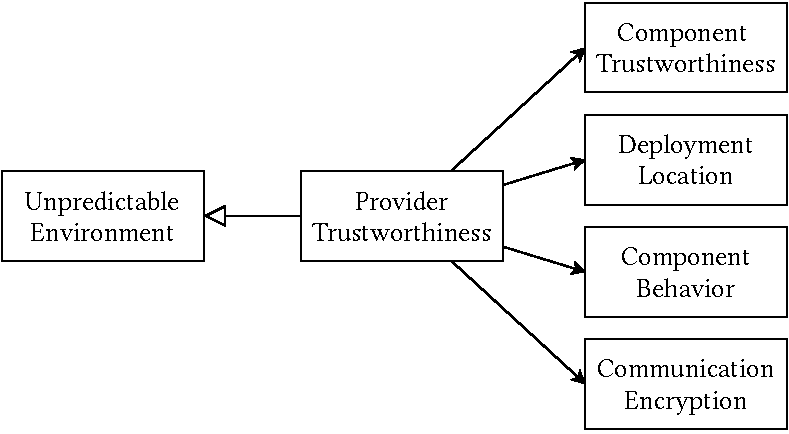
\includegraphics[width=0.8\linewidth]{figures/chapter5/arc3n-relations.pdf}
    \caption{Uncertainty source about the \enquote{Provider Trustworthiness} with its parent uncertainty source \enquote{Unpredictable Environment} and related uncertainties.}
    \label{fig:classification:identification:uncertaintygraph}
\end{figure}

In addition to its own properties, classification, examples, and keywords, \emph{Uncertainty Sources} can have relations and parent uncertainties.
In our example, \emph{Provider Trustworthiness} is a child of the uncertainty source \emph{Unpredictable Environment} \cite{ramirez_taxonomy_2012}, and related to uncertainty sources of our initial population regarding encrypted communication, component trustworthiness, and deployment location.
This is illustrated in \autoref{fig:classification:identification:uncertaintygraph}.

Combined, this information provides comprehensive context knowledge for software architects, raises awareness, and simplifies the assessment.
By attaching this information and also linking related uncertainty types, we address the organizational challenges of collecting uncertainty sources and enable to search and filter for uncertainty sources.
Additionally, there are no space limitations regarding examples, visualizations, and discussions.
To demonstrate this, we enriched 51 uncertainty sources from multiple classifications \cite{hahner_classification_2023,ramirez_taxonomy_2012} with context information, examples, and also uncertainty relations and inheritance as part of our data set \cite{dataset}.
In sum, this addresses Problem \PR{1}{4} and enables non-experts to reuse expert knowledge on uncertainty sources.

Note that the current state of research cannot create a generally applicable and comprehensive answer to identifying all possible uncertainty sources \cite{weyns_towards_2023}.
However, processing, persisting and relating information about uncertainty sources provides a pragmatic first step, especially for practitioners \cite{hahner_arcn_2024}.
To this end, approaches like this uncertainty source catalog are steps towards also addressing unanticipated changes that are not totally unforeseeable \cite{garlan_software_2010}.
Following the discussion about the orders of uncertainty \cite{armour_five_2000}, we hereby lower the order of uncertainty from the \emph{third} to the \emph{second} order. 
Although there can be a lack of awareness of an individual, we provide means to identify some uncertainty sources, which previously were unknown to this individual \cite{perez-palacin_uncertainties_2014}.

\finding{Knowledge about uncertainty sources can be reused across software architectures. 
Extending the classification of uncertainty sources with descriptions, examples, keywords, and relations between uncertainty sources helps in the identification and simplifies the assessment.
This reuse of expert knowledge addresses the \acf{UAP} and helps to deal with the ever-present challenge of unanticipated change.}





\section{A Collaborative Approach for Uncertainty Catalogs}%
\label{sec:classification:collaboration}

Our classification presented in \autoref{sec:classification:classification} provides the terminology to understand and discuss uncertainty sources, and the catalog meta model presented in \autoref{sec:classification:identification} simplifies the identification of relevant uncertainty sources and sharing of knowledge.
However, to be applicable, knowledge reuse must be simplified and should not be limited to individuals or institutions.
With Problem \PR{1}{5}, we stressed the importance of an open and publicly available catalog of uncertainty sources.
Collecting uncertainty sources only within publications \cite{ramirez_taxonomy_2012} or data sets \cite{hahner_classification_2023} lacks reusability, extensibility, and availability.
To address this, we propose a web-based catalog approach in the following.

\begin{figure}
    \centering
    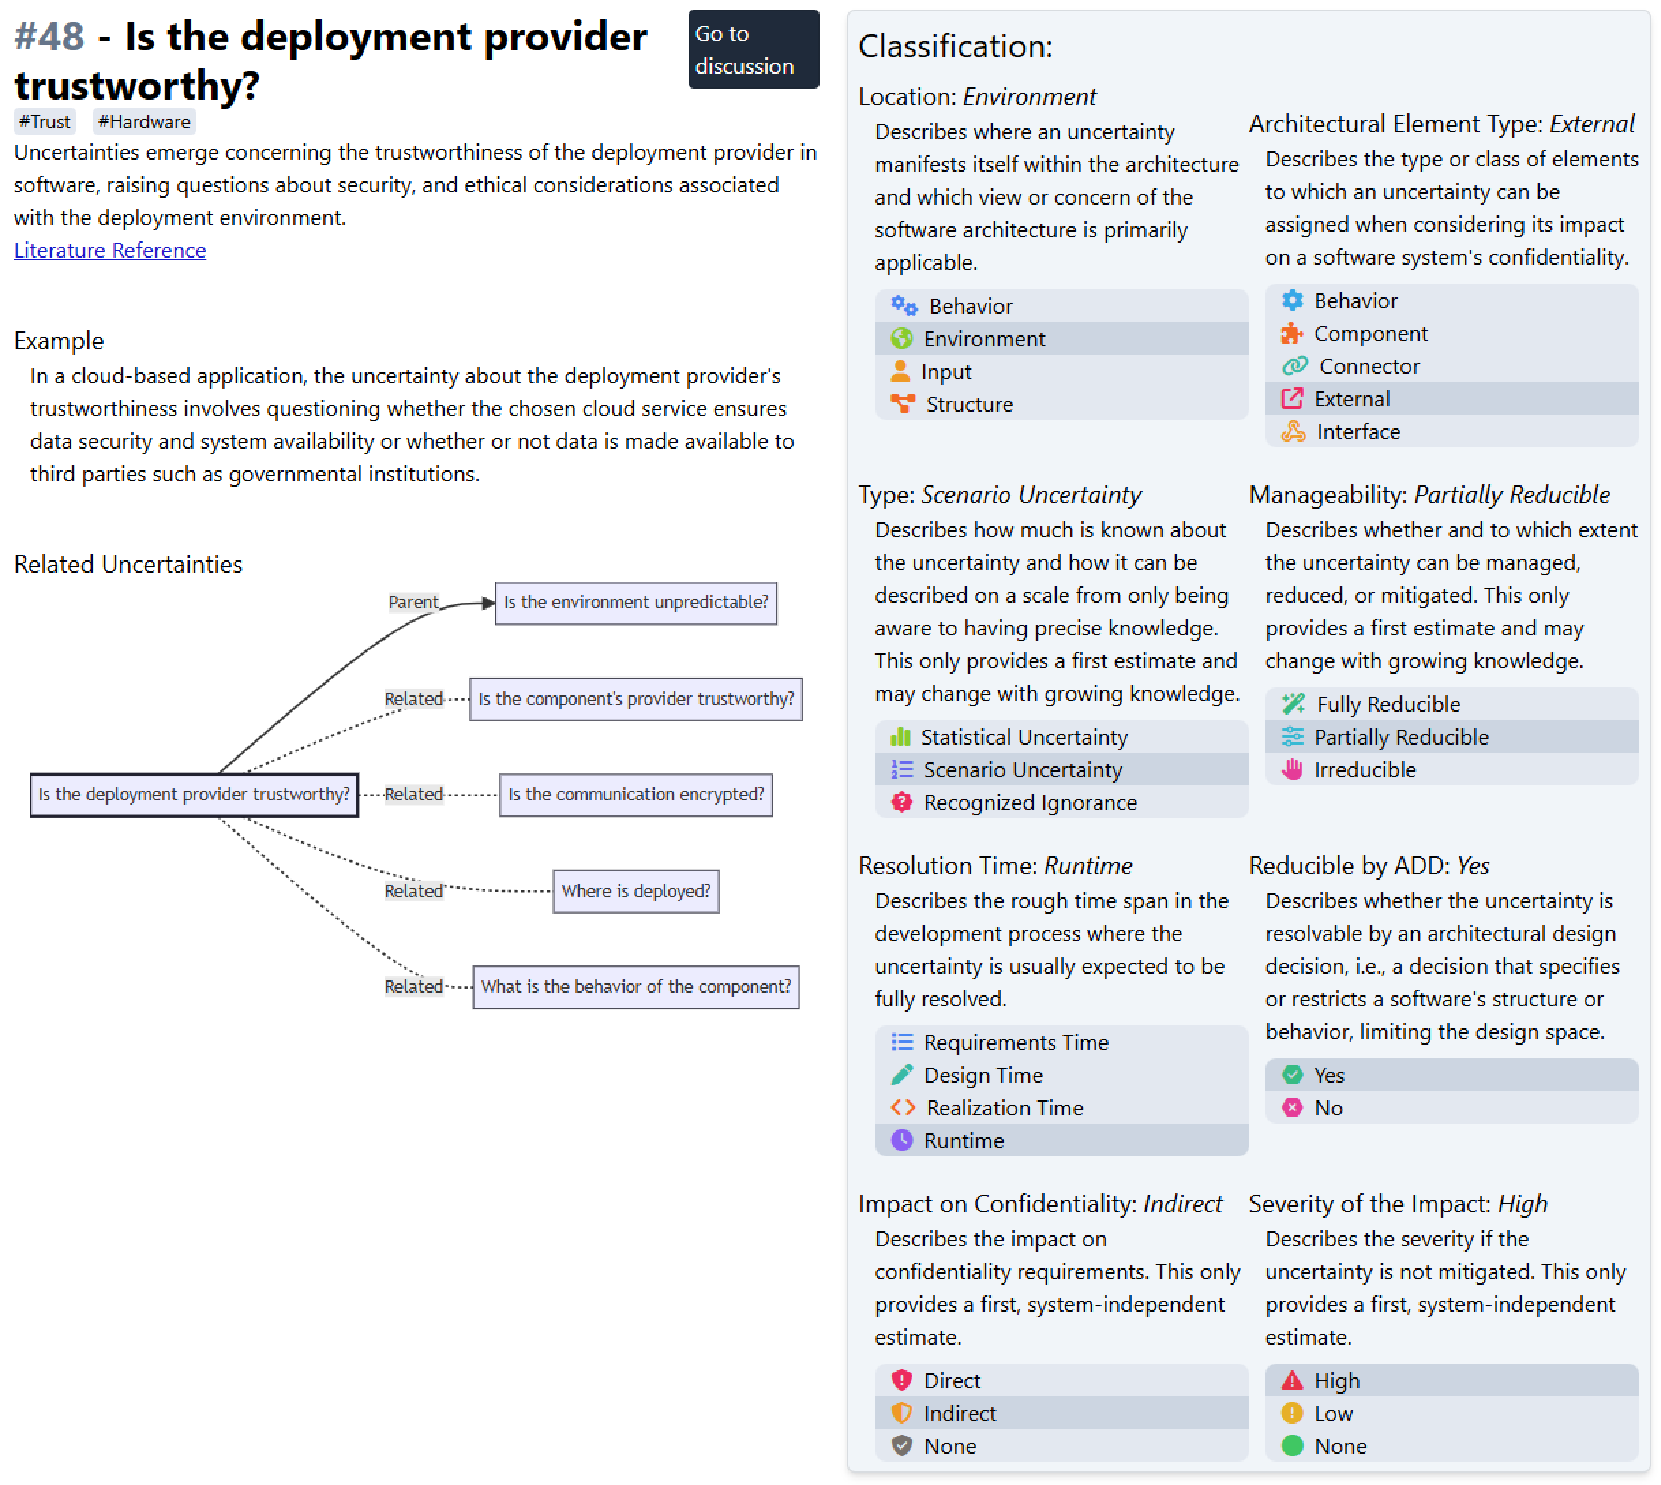
\includegraphics[width=\linewidth]{figures/chapter5/arc3n-screenshot.pdf}
    \caption[Screenshot of the detail view of our tooling.]{Screenshot of the detail view of our tooling \arcen. It shows the description, explanation, and classification of the uncertainty source regarding the trustworthiness of a resource provider.}
    \label{fig:classification:collaboration:screenshot}
\end{figure}

We realized our meta model and catalog approach as \textbf{\arcen}, which stands for \emph{Rese\textbf{arc}h \textbf{arc}hive for Software-\textbf{Arc}hitectural U\textbf{n}certainty}\footnote{\arcen is open-source and available online: \url{https://arc3n.abunai.dev/}. It is also archived in our data set \cite{dataset}. Any similarities by name with extensively praised jewels are completely coincidental.}.
Our tooling revolves around a table of uncertainty sources and their classification which allows for quick navigation, search, and filtering by keywords or classification categories.
By selecting a source, software architects can see its description, examples, related sources, and its classification.
Because there is no space limitation, the selected options of the classification can be explained in detail, as shown in \autoref{fig:classification:collaboration:screenshot}.
We also provide further explanation of all classification categories and relate known uncertainty sources similar to \autoref{fig:classification:identification:uncertaintygraph}.
Software architects can quickly navigate through uncertainty sources, examples, and classification.
Last, the full catalog can be downloaded in a machine-readable \ac{JSON} format.

All four uncertainty sources of our running example are contained in the initial population of our catalog.
Thus, security experts could become aware of these uncertainty sources by using our tool support.
To identify the uncertainty of the provider's trustworthiness (\U{4}), they could search for trust-related uncertainty sources or navigate to this uncertainty by its related uncertainty sources, e.g., the unpredictable environment or the encrypted communication.
They could even identify the uncertainty by investigating the open deployment decision with Uncertainty \U{3} as both uncertainty sources are related.

We chose a web-based approach to minimize the effort required to set up and use the tooling.
We use a GitHub \cite{GitHub2024} git repository as the backend for adding new uncertainty sources as well as discussions between participants.
New uncertainty sources can be added directly from within our tool support and are then retrieved by using the open GitHub API \cite{GitHub2024}.
This enables lightweight and openly accessible storage of all required information.
We choose GitHub to minimize the risk of link decay, which is especially prominent on institutional websites \cite{goh_link_2007}.
The information retrieval is automated using a DevOps pipeline based on GitHub Actions \cite{GitHub2024}.
Once the information has been updated, our tooling works completely autonomously and can be self-hosted or used locally.
This enables the easy integration of other information sources and also simplifies switching to other platforms like GitLab.

Our tooling \arcen collects uncertainty sources in a central place instead of relying only on publication-based collections which simplifies the collaboration of researchers and practitioners.
We foster two types of collaboration: \arcen benefits the communication between different roles with different knowledge, e.g., security experts and software architects. 
It also benefits peers with the same role as a shared catalog for exchange and documentation.
New uncertainty sources can be proposed by everyone based on the open-source GitHub repository.
All required information is stored as part of the tool support and can be downloaded in third-party analyses.
In sum, this approach provides an easy-to-use, extensible, and open collaborative approach to address Problem \PR{1}{5}.
Note that we do not claim comprehensiveness regarding uncertainty sources with this catalog.
We do also not claim long-term availability over decades.
Nevertheless, this approach is a proposal towards an open and available catalog to foster collaboration \cite{sterz_intelligente_2022}.





\section{Assumptions and Limitations}%
\label{sec:classification:limitations}

In this section, we discuss the assumptions and limitations of the identification and classification approaches presented in this chapter.
We partition these into five groups: The focus on confidentiality, the use of software architecture-based approaches at design time, the lack of automated analysis, the cooperation required for collaborative approaches, and the ever-present challenge of unanticipated change.

\paragraph{Focus on confidentiality}
First, we only focus on confidentiality as a central quality attribute of our classification.
While this reduces the generalizability, we do this intentionally to obtain more precise results for the modeling and analysis of uncertainty sources.
As demonstrated, the focus on confidentiality enables the connection of the uncertainty types to \acp{DFD}, which simplifies later data flow-based confidentiality analysis.
Additionally, we assume that the concepts can at least be applied partially to related quality attributes like integrity \cite{boltz_extensible_2024,seifermann_architectural_2022}.
Using the location as a central classification category and representing uncertainty in flow diagrams were the inspirations for other work \cite{acosta_uncertainty_2022,camara_uncertainty_2024}.
Nevertheless, we do not claim generalizability beyond confidentiality.

\paragraph{Using the software architectural abstraction}
Similarly, we limit ourselves to software-architectural uncertainty, as defined in \autoref{sec:classification:relation}.
This was also an explicit decision due to fit existing modeling \cite{reussner_modeling_2016,seifermann_unified_2021} and analysis \cite{seifermann_data-driven_2019,seifermann_detecting_2022,tuma_flaws_2019} approaches for confidentiality.
Still, most categories are general enough to be used even without explicit models, e.g., \emph{Type}, \emph{Manageability}, or \emph{Resolution Time}.
We assume that software architects and security experts already have enough knowledge about the software system to assess uncertainty at design time.
Such assumptions exist in many architecture-based analyses \cite{seifermann_architectural_2022,walter_context-based_2023}.

\paragraph{Transitive impact of uncertainty}
Third, the approaches for identification and classification provide no assistance for the transitive impact of uncertainty.
The uncertainty source is often not the location where the uncertainty affects confidentiality and where it can be mitigated.
We presented the relation of uncertainty sources and their impact in \autoref{sec:classification:relation}, e.g., with the transitive impact of the Uncertainty \U{1} about the user input to the \emph{Database Service} shown in \autoref{fig:classification:example}.
However, to face such propagation effects, a precise description of uncertainty---such as our classification---is required in the first place.
Additionally, the modeling and analysis of uncertainty for design-time confidentiality analysis require tool support as \enquote{detecting confidentiality issues manually is not feasible} \cite{seifermann_data-driven_2019}.
We will address this limitation in the following chapters.

\paragraph{Collaboration for joint uncertainty catalogs}
Our web-based approach \arcen represents a publicly available uncertainty catalog.
Here, we assume that researchers and practitioners alike benefit from sharing knowledge about uncertainty sources, as known from legal sciences \cite{sterz_intelligente_2022}. 
However, companies or institutions could try to keep the information private, especially regarding sensitive topics like security.
The lack of willingness to cooperate limits the benefits of a shared knowledge base.
Nevertheless, \arcen could also be used in a closed environment but with limited usefulness.

\paragraph{Unanticipated change}
We do not claim to have solved the challenge of unanticipated change.
A recently published research agenda \cite{weyns_towards_2023} names the challenge of end-to-end approaches that can operate in changing real-world conditions.
We do not provide a solution to such unanticipated change.
However, our identification approach represents a pragmatic approach towards reducing the effect to the individual by sharing knowledge about them, i.e., making them known.
In sum, our catalog approach can be seen as a first step or a potential part of a comprehensive solution.





\section{Summary and Outlook}%
\label{sec:classification:summary}

In this chapter, we presented our classification of \emph{software-architectural uncertainty} and our approach to address the identification of uncertainty.
This represents our first Contribution \C{1} and provides the answer to \RQ{1}.

First, we presented our understanding of the relation of uncertainty, confidentiality, and software architecture to address Problem \PR{1}{1}.
We highlighted the distinction between an uncertainty source and its impact.
The former represents the origin of uncertainty in the software system or its environment while the latter represents the actual location of the impact of the uncertainty source on confidentiality.
We also related the notion of uncertainty to the terminology known from \acfp{SAS} \cite{weyns_introduction_2020}, the \emph{cone of uncertainty} \cite{mcconnell_software_1998}, and \acfp{ADD} \cite{kruchten_ontology_2004,jansen_software_2005}.

Based on this discussion, we investigated existing uncertainty classifications \cite{walker_defining_2003,perez-palacin_uncertainties_2014,ramirez_taxonomy_2012,mahdavi-hezavehi_classification_2017,bures_capturing_2020} and defined our own classification tailored to the impact on confidentiality, thereby addressing Problem \PR{1}{2}.
Our classification contains 8 categories with a total of 27 options.
They classify uncertainty in categories like location, manageability, or resolution time.
The central category is the \emph{Architectural Element Type} as this category describes where to annotate an uncertainty source in architectural models.
Last, we illustrated the classification using our running example.

Building on this classification, we addressed Problem \PR{1}{3} of representing uncertainty as a first-class concern in \acp{DFD}.
Our first finding was that the five uncertainty types of the aforementioned classification match the model elements of \acp{DFD}.
We then partitioned the five uncertainty types category into \emph{primary} and \emph{secondary} uncertainty.
This enables a simple and straightforward representation of uncertainty in \acp{DAG}, which can be used to represent \acp{DFD}.
Primary uncertainty affects vertices, and secondary uncertainty affects edges between vertices.

Afterward, we extended the classification and presented a meta model for \emph{uncertainty source catalogs}, which addresses Problem \PR{1}{4}.
We proposed the enrichment of classified uncertainty sources with descriptions, keywords, and examples.
Additionally, uncertainty sources are usually not independent \cite{camara_addressing_2022} and thus can have relations and inheritance.
By collecting such information in a central archive, the \ac{UAP} can be partially addressed.

Last, we presented our tooling \arcen to create an open catalog of uncertainty sources and to address Problem \PR{1}{5}.
Our initial population contains 51 uncertainty sources with descriptions, examples, and relations.
It is publicly available under an open-source license and can help to identify relevant uncertainty sources that were previously unknown to security experts.
By combining classification and identification, we support the first two activities presented in \autoref{sec:overview:procedure}.

\RQ{1} asked about the identification, description, and classification of software-architectural uncertainty regarding confidentiality.
Our comprehensive answer to this question comprises the inspection of existing classifications and the definition of a novel classification regarding the impact of uncertainty on confidentiality.
We derive five uncertainty types that fit \acp{DFD}, which are often used to analyze confidentiality \cite{seifermann_unified_2021}.
By applying these uncertainty types to \acp{DAG}, we close the gap between uncertainty sources and confidentiality.
Furthermore, our classification provides the means to describe and discuss uncertainty.
By extending the classification to form tool-supported uncertainty source catalogs, we ultimately also address the question of description and identification.

The benefits of our Contribution \C{1} include precise terminology to discuss and understand uncertainty regarding confidentiality.
This supports both software architects and security experts in modeling and analyzing software-intensive systems.
As proposed in \autoref{ch:overview}, we do not require an additional \emph{uncertainty expert} role, as the required knowledge is contained in the classification and the uncertainty source catalog.
Here, our tooling \arcen presents a useful starting point.
By identifying and assessing uncertainty sources early, the reasoning and prioritization of \acp{ADD} is simplified and costly backtracking is minimized.
This is especially true regarding uncertainty interactions \cite{camara_addressing_2022}, which represent uncertainty impacts that are particularly hard to find and mitigate.
Last, our classification lays the foundations for further integration of software-architectural uncertainty in the architecture-based analysis of confidentiality.

We will revisit the idea of representing uncertainty sources and their impact as first-class entities in \acp{DFD} and \acp{DAG} in the following chapters.
In \readingpath{ch:impactanalysis}, we discuss uncertainty propagation in architectural models and \acp{DFD} alike.
This will help to better understand the actual impact of uncertainty sources on confidentiality beyond the early assessment using our classification.
This also addresses the limitation of the sole classification regarding the transitive impact of uncertainty.
It also defines the foundations for later uncertainty-aware analysis in \readingpath{ch:confidentialityanalysis}.
Here, we will also see again the distinction between primary and secondary uncertainty and how it can be used to speed up data flow analysis.
Last, the evaluation of this chapter will be presented in \readingpath{ch:evaluation}.





\section{In Simpler Words}%
\label{sec:classification:simple}

In this chapter, we focus on two things: The classification and the identification of uncertainty.
This is an important first step because we first need to better understand the threat to confidentiality, which is uncertainty.
We define clear terms for software architects and security experts in the form of a classification.
Afterward, we show how to extend this classification in order to identify more uncertainty sources.

A classification helps to understand important properties of a classified element---in our case, uncertainty.
Many researchers already defined many classifications of uncertainty.
However, they do not fit our purpose, relating uncertainty to confidentiality.
Thus, we define our own classification based on the existing ones.
We propose different categories like the location, the manageability, or the severity of the impact.
For instance, the uncertainty regarding user behavior can be located in the system input as users operate a software system.
We cannot control their input but we can try to think of possible behavior in advance and thus partially reduce this uncertainty.
If the user behaves maliciously and tries to attack our system, the severity of the impact can be high.
In total, we define eight categories like these three.
They help us to better understand uncertainty, and group uncertainty sources together.
We apply this knowledge to data flow diagrams, a diagram type that is often used to reason about confidentiality.
By connecting this uncertainty terminology to data flow diagrams, we lay the foundations for the automated analyses we will present in the following chapters.

To help software architects and security experts even more, we also discuss how to identify uncertainty sources.
If you had not read the previous paragraph, you might not have known about the uncertainty of the user's behavior.
This is the nature of unexpected changes---often, you do not even know that you do not know about the change.
But now that I told you, you know about the uncertainty of user behavior.
You still do not know how the user will behave in the end, but you are at least aware of the issue.
We present a software tool that helps to collect uncertainty sources and make software architects and security experts aware of them.
This also helps to connect different uncertainty sources, as they often have relations.
For instance, if we apply input validation to address the uncertain user input, we can address this uncertainty.
But if we do not know how this input validation works and whether it always works correctly, the validation itself is an uncertainty source.
Then, both uncertainties are connected---this is called \emph{uncertainty interaction}.
Uncertainty interactions are particularly dangerous and hard to find.
Our contribution regarding the identification and classification can also help here.
